\documentclass[11pt,border=4pt]{standalone}
% Estilo comum dos fluxogramas do Caderno C3 (cores do modelo do MOP)
\usepackage[T1]{fontenc}
\usepackage[utf8]{inputenc}
\usepackage{helvet}
\renewcommand{\familydefault}{\sfdefault}
\usepackage{amssymb}
\usepackage{tikz}
\usetikzlibrary{positioning, arrows.meta, shapes.geometric, shapes.symbols, shapes.misc,
  calc, fit, backgrounds, decorations.pathmorphing, patterns, shadows}
% Paleta do modelo do caderno
\definecolor{cTeal}{HTML}{00747A}
\definecolor{cNavy}{HTML}{0B3A5A}
\definecolor{cBlue}{HTML}{0A73BA}
\definecolor{cBlueBg}{HTML}{EBF4F9}
\definecolor{cTealBg}{HTML}{E3F1F2}
\definecolor{cTealMid}{HTML}{9CCFD2}
\definecolor{cGrayBg}{HTML}{F2F2F2}
\definecolor{cGrayLine}{HTML}{BFBFBF}
\definecolor{cGrayText}{HTML}{595959}
\definecolor{cText}{HTML}{1A1A1A}
\definecolor{cAmber}{HTML}{B7791F}
\definecolor{cAmberBg}{HTML}{FDF3DC}
\definecolor{cGreen}{HTML}{3D7D3A}
\definecolor{cGreenBg}{HTML}{E8F2E4}
\color{cText}
\tikzset{
  every node/.style={font=\footnotesize, text=cText},
  etapa/.style={draw=cTeal, fill=cTealBg, rounded corners=2pt, align=center,
     inner sep=3.5pt, minimum height=0.85cm, text width=#1, line width=0.6pt},
  etapa/.default={3.2cm},
  marco/.style={draw=cNavy, fill=cNavy, rounded corners=2pt, align=center,
     inner sep=3.5pt, minimum height=0.85cm, text width=#1,
     font=\footnotesize\bfseries, text=white},
  marco/.default={3.2cm},
  marcoteal/.style={draw=cTeal, fill=cTeal, rounded corners=2pt, align=center,
     inner sep=3.5pt, minimum height=0.85cm, text width=#1,
     font=\footnotesize\bfseries, text=white},
  marcoteal/.default={3.2cm},
  externo/.style={draw=cGrayLine, fill=cGrayBg, rounded corners=2pt, align=center,
     inner sep=3.5pt, minimum height=0.85cm, text width=#1},
  externo/.default={3.2cm},
  produto/.style={draw=cTeal!70, fill=white, rounded corners=1pt, align=center,
     inner sep=2.5pt, minimum height=0.6cm, text width=#1, font=\scriptsize},
  produto/.default={2.4cm},
  decisao/.style={draw=cAmber, fill=cAmberBg, diamond, aspect=2, align=center,
     inner sep=1pt, font=\scriptsize, line width=0.6pt},
  correcao/.style={draw=cAmber, fill=cAmberBg, rounded corners=2pt, align=center,
     inner sep=3pt, minimum height=0.8cm, text width=#1, font=\scriptsize},
  correcao/.default={2.6cm},
  transversal/.style={draw=cBlue, fill=cBlueBg, dashed, rounded corners=2pt, align=center,
     inner sep=3.5pt, text width=#1, line width=0.6pt},
  transversal/.default={6cm},
  seta/.style={-{Stealth[length=2.2mm,width=1.8mm]}, line width=0.8pt, draw=cNavy},
  setaleve/.style={-{Stealth[length=1.8mm,width=1.5mm]}, line width=0.6pt, draw=cGrayText},
  setatracejada/.style={-{Stealth[length=2mm]}, line width=0.7pt, dashed, draw=cGrayText},
  rotulo/.style={font=\scriptsize\itshape, text=cGrayText, fill=white, inner sep=1pt},
  fase/.style={signal, signal to=east, signal from=west, draw=cTeal, fill=cTealBg,
     align=center, font=\scriptsize\bfseries, minimum height=1.05cm, text width=#1,
     inner sep=2pt},
  fase/.default={1.9cm},
  raia/.style={draw=cGrayLine, fill=cGrayBg, minimum width=#1, minimum height=0.9cm,
     anchor=north west},
  tituloraia/.style={font=\scriptsize\bfseries, text=cNavy, align=center, text width=1.75cm},
  cab/.style={font=\scriptsize\bfseries, text=white, fill=cNavy, align=center,
     inner sep=3pt, text width=#1, minimum height=0.6cm},
  cab/.default={3cm},
  bloco/.style={draw=cGrayLine, fill=cGrayBg, rounded corners=3pt},
}
% sem hifenização nas caixas dos fluxogramas
\AtBeginDocument{\hyphenpenalty=10000 \exhyphenpenalty=10000 \sloppy}

\begin{document}

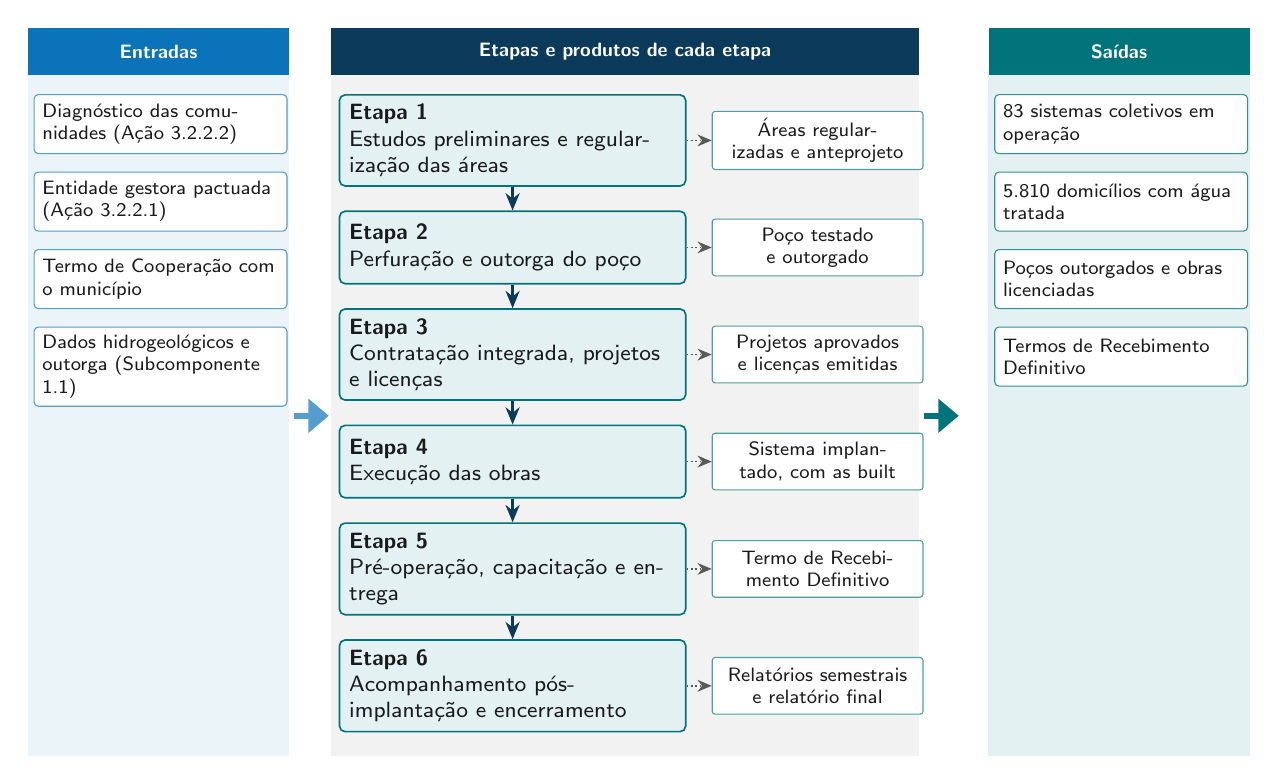
\begin{tikzpicture}

  \tikzset{
    item/.style={draw=#1, fill=white, rounded corners=1.5pt, align=left, text width=3.0cm,
      inner sep=3pt, font=\scriptsize, minimum height=0.75cm},
    passo/.style={etapa=4.15cm, minimum height=0.92cm, align=left},
    chip/.style={produto=2.5cm, minimum height=0.72cm}
  }
  \node[cab=3.1cm, fill=cBlue, anchor=north west] (hE) at (0,0) {Entradas};
  \node[cab=7.25cm, fill=cNavy, anchor=north west] (hP) at (3.85,0) {Etapas e produtos de cada etapa};
  \node[cab=3.1cm, fill=cTeal, anchor=north west] (hS) at (12.2,0) {Saídas};

  \node[passo, anchor=north west] (e1) at (3.95,-0.85) {\textbf{Etapa 1}\\ Estudos preliminares e regularização das áreas};
  \node[chip, anchor=west] (p1) at ($(e1.east)+(0.32,0)$) {Áreas regularizadas e anteprojeto};
  \draw[setaleve, densely dotted] (e1.east) -- (p1.west);
  \node[passo, below=0.3cm of e1] (e2) {\textbf{Etapa 2}\\ Perfuração e outorga do poço};
  \node[chip, anchor=west] (p2) at ($(e2.east)+(0.32,0)$) {Poço testado e outorgado};
  \draw[setaleve, densely dotted] (e2.east) -- (p2.west);
  \draw[seta] (e1.south) -- (e2.north);
  \node[passo, below=0.3cm of e2] (e3) {\textbf{Etapa 3}\\ Contratação integrada, projetos e licenças};
  \node[chip, anchor=west] (p3) at ($(e3.east)+(0.32,0)$) {Projetos aprovados e licenças emitidas};
  \draw[setaleve, densely dotted] (e3.east) -- (p3.west);
  \draw[seta] (e2.south) -- (e3.north);
  \node[passo, below=0.3cm of e3] (e4) {\textbf{Etapa 4}\\ Execução das obras};
  \node[chip, anchor=west] (p4) at ($(e4.east)+(0.32,0)$) {Sistema implantado, com as built};
  \draw[setaleve, densely dotted] (e4.east) -- (p4.west);
  \draw[seta] (e3.south) -- (e4.north);
  \node[passo, below=0.3cm of e4] (e5) {\textbf{Etapa 5}\\ Pré-operação, capacitação e entrega};
  \node[chip, anchor=west] (p5) at ($(e5.east)+(0.32,0)$) {Termo de Recebimento Definitivo};
  \draw[setaleve, densely dotted] (e5.east) -- (p5.west);
  \draw[seta] (e4.south) -- (e5.north);
  \node[passo, below=0.3cm of e5] (e6) {\textbf{Etapa 6}\\ Acompanhamento pós-implantação e encerramento};
  \node[chip, anchor=west] (p6) at ($(e6.east)+(0.32,0)$) {Relatórios semestrais e relatório final};
  \draw[setaleve, densely dotted] (e6.east) -- (p6.west);
  \draw[seta] (e5.south) -- (e6.north);
  \coordinate (fundo) at ($(e6.south)+(0,-0.3)$);
  \node[item=cBlue!70, anchor=north west] (i1) at (0.075,-0.85) {Diagnóstico das comunidades (Ação 3.2.2.2)};
  \node[item=cBlue!70, below=0.22cm of i1] (i2) {Entidade gestora pactuada (Ação 3.2.2.1)};
  \node[item=cBlue!70, below=0.22cm of i2] (i3) {Termo de Cooperação com o município};
  \node[item=cBlue!70, below=0.22cm of i3] (i4) {Dados hidrogeológicos e outorga (Subcomponente 1.1)};
  \node[item=cTeal!80, anchor=north west] (o1) at (12.275,-0.85) {83 sistemas coletivos em operação};
  \node[item=cTeal!80, below=0.22cm of o1] (o2) {5.810 domicílios com água tratada};
  \node[item=cTeal!80, below=0.22cm of o2] (o3) {Poços outorgados e obras licenciadas};
  \node[item=cTeal!80, below=0.22cm of o3] (o4) {Termos de Recebimento Definitivo};

  \begin{scope}[on background layer]
    \fill[cBlueBg] (hE.south west) rectangle (hE.east |- fundo);
    \fill[cGrayBg] (hP.south west) rectangle (hP.east |- fundo);
    \fill[cTealBg] (hS.south west) rectangle (hS.east |- fundo);
  \end{scope}
  \coordinate (meio) at ($(hP.south)!0.5!(hP.south |- fundo)$);
  \draw[-{Triangle[length=2.6mm,width=4.2mm]}, line width=2.2pt, draw=cBlue!70]
    (hE.east |- meio) ++(0.06,0) -- ++(0.44,0);
  \draw[-{Triangle[length=2.6mm,width=4.2mm]}, line width=2.2pt, draw=cTeal]
    (hP.east |- meio) ++(0.06,0) -- ++(0.44,0);
\end{tikzpicture}

\end{document}
